% Copyright (c) 2024 by the University of Waikato, Hamilton, NZ. 
% This work is made available under the terms of the 
% Creative Commons Attribution-ShareAlike 4.0 license,
% http://creativecommons.org/licenses/by-sa/4.0/.

\documentclass[a4paper]{book}

\usepackage{wrapfig}
\usepackage{graphicx}
\usepackage{hyperref}
\usepackage{multirow}
\usepackage{scalefnt}
\usepackage{tikz}
\usepackage{varwidth}

% watermark -- for draft stage
\usepackage[firstpage]{draftwatermark}
\SetWatermarkLightness{0.9}
\SetWatermarkScale{5}

% This work is made available under the terms of the
% Creative Commons Attribution-ShareAlike 4.0 license,
% http://creativecommons.org/licenses/by-sa/4.0/.
%
% Version: $Revision: 2916 $

\newenvironment{tight_itemize}{
\begin{itemize}
  \setlength{\itemsep}{1pt}
  \setlength{\parskip}{0pt}
  \setlength{\parsep}{0pt}}{\end{itemize}
}

\newenvironment{tight_enumerate}{
\begin{enumerate}
  \setlength{\itemsep}{1pt}
  \setlength{\parskip}{0pt}
  \setlength{\parsep}{0pt}}{\end{enumerate}
}

% if you just need a simple heading
% Usage:
%   \heading{the text of the heading}
\newcommand{\heading}[1]{
  \vspace{0.3cm} \noindent \textbf{#1} \newline
}

\newcommand{\icon}[1]{\tikz[baseline=-3pt]\node[inner sep=0pt,outer sep=0pt]{\includegraphics[height=1.1em]{#1}};}


\title{
  \textbf{ADAMS} \\
  {\Large \textbf{A}dvanced \textbf{D}ata mining \textbf{A}nd \textbf{M}achine
  learning \textbf{S}ystem} \\
  {\Large Module: adams-git} \\
  \vspace{1cm}
  
\includegraphics[width=2cm]{images/git-module.png} \\
}
\author{
  Peter Reutemann
}

\setcounter{secnumdepth}{3}
\setcounter{tocdepth}{3}

\begin{document}

\begin{titlepage}
\maketitle

\thispagestyle{empty}
\center
\begin{table}[b]
	\begin{tabular}{c l l}
		\parbox[c][2cm]{2cm}{\copyright 2024} &
		\parbox[c][2cm]{5cm}{
\includegraphics[width=5cm]{images/coat_of_arms.pdf}} \\
	\end{tabular}
	
\includegraphics[width=12cm]{images/cc.png} \\
\end{table}

\end{titlepage}

\tableofcontents
\listoffigures
%\listoftables


%%%%%%%%%%%%%%%%%%%%%%%%%%%%%%%%%%%
\chapter{Introduction}
\textit{git} is an is a free and open source distributed version control system designed to handle everything
from small to very large projects with speed and efficiency\cite{git}.

\section{Preferences}
The \textit{Git} section in the global preferences (see Figure \ref{preferences}) allows you to modify
the git support within ADAMS.

\noindent Some notes:
\begin{tight_itemize}
    \item \textit{SshDir} - where to find your ssh keys
    \item \textit{KnownHosts} - the file that lists the public keys of your known hosts
    \item \textit{User} and \textit{Email} can be used to override the settings from your \texttt{.gitconfig} file\cite{git-config}.
    \item \textit{LoggingLevel} - whether you want to see any logging output
    \item \textit{FlowEditorSupport} - if ticked, enables a \textit{Git} sub-menu in the Flow editor
\end{tight_itemize}

\begin{figure}[htb]
  \centering
  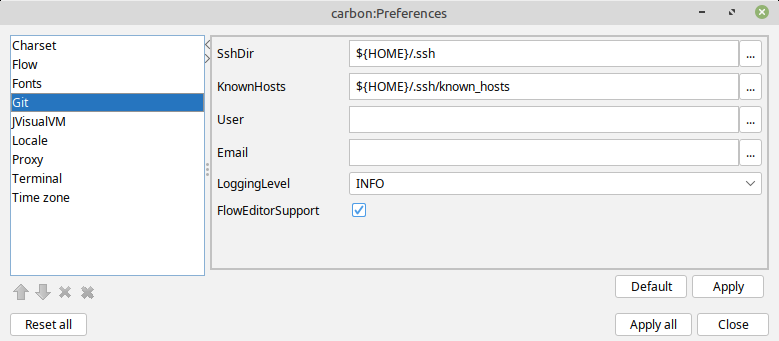
\includegraphics[width=12.0cm]{images/preferences.png}
  \caption{Git preferences}
  \label{preferences}
\end{figure}


\section{Flow editor}
With support enabled in the global \textit{Preferences} (off by default), you get the following
additional sub-menu in the Flow editor: \textit{File $\rightarrow$ Git}

Assuming that your flows are being saved in a directory structure that is part of a git
repository (local or clone from remote), then you can do the following:
\begin{tight_itemize}
    \item \textit{Add} -- adds the flow to the files that are being tracked by git
    \item \textit{Commit} -- prompts you to enter a message to associate the commit of this flow;
    if \textit{User} or \textit{Email} have not been defined, then you will get prompted
    for these as well (see \cite{git-config})
    \item \textit{Log} -- compiles the log for the flow
    \item \textit{Pull} -- allows pulling in changes from the remote origin (not enabled for local repositories)
    \item \textit{Push} -- allows pushing out your changes to the remote origin (not enabled for local repositories)
    \item \textit{Rollback} -- reverts changes to local files or adding files to git
    \item \textit{Reset session} -- clears the session cache
\end{tight_itemize}


%%%%%%%%%%%%%%%%%%%%%%%%%%%%%%%%%%%
% This work is made available under the terms of the 
% Creative Commons Attribution-ShareAlike 4.0 license,
% http://creativecommons.org/licenses/by-sa/4.0/.

\begin{thebibliography}{999}
	% to make the bibliography appear in the TOC
	\addcontentsline{toc}{chapter}{Bibliography}

    % references
	\bibitem{adams}
		\textit{ADAMS} -- Advanced Data mining and Machine learning System \\
		\url{https://adams.cms.waikato.ac.nz/}{}

	\bibitem{djl}
		\textit{Deep Java Library} -- open source library to build and deploy deep learning in Java. \\
		\url{https://djl.ai/}{}

\end{thebibliography}


\end{document}
